% !TEX program = lualatex
\documentclass[11pt]{article}

% -------- LuaLaTeX : polices et langue --------
\usepackage{fontspec}
\setmainfont{Latin Modern Roman}
\setsansfont{Tex Gyre Heros}
%\renewcommand{\familydefault}{\sfdefault} % force le sans serif par défaut
\usepackage{polyglossia}
\setdefaultlanguage{french}

% -------- Mise en page --------
\usepackage[a4paper,margin=1cm]{geometry}
\usepackage{multicol}
\usepackage{fancyhdr}
\pagestyle{empty}
\usepackage[most]{tcolorbox}

% -------- Mathématiques --------
\usepackage{amsmath,amssymb,mathtools}
% \usepackage{siunitx}
% \sisetup{locale=FR}

\usepackage{enumitem}
\setlist[itemize]{left=0pt}
\setlist[enumerate]{left=0pt, label=\textbf{\arabic*}.}

\usepackage{ProfCollege}
\usepackage{ProfMaquette}

%\usepackage{tabularray}
\usepackage{tabularx}

% -------- Divers --------
\newcommand{\ligne}{{\color{gray!60}\hrulefill}}

\setlength{\parindent}{0pt}

\begin{document}



\begin{Maquette}[DM]{
        Numero = 1, Code={}, Date = Lundi 6 octobre 2025, Niveau = Troisième
    }

    \emph{Ce travail est à rédiger sur une feuille. Le sujet est à coller, plié, au dos de votre copie.}

    \begin{exercice}
        \brm{6}
        Voici les notes obtenues par une classe au dernier contrôle de mathématiques :
         \begin{center}
                      \renewcommand{\arraystretch}{1.2}
                      \begin{tabular}{|*{23}{c|}}
                          \hline
                     19	& 7&	11&	10&	16&	12&	11&	10&	16&	10&	10&	18&	20&	9&	5&	19&	10&	7&	19&	16&	17&	15&	12        \\
                          \hline
                      \end{tabular}
                  \end{center}
       
        \begin{enumerate}
            \item Calculer la moyenne des notes des élèves de cette classe.
            \item Calculer l’étendue de cette série de note.
            \item Déterminer la note médiane de la classe.
            \item Recopier et compléter le tableau suivant.
            \begin{center}
                      \renewcommand{\arraystretch}{1.2}
                      \begin{tabular}{|*{4}{c|}}
                          \hline
                          \textbf{Note}&5&7&\ldots \\ \hline
                          \textbf{Effectif}&1&2&\ldots \\
                          \hline
                      \end{tabular}
                  \end{center}
            \item Représenter ci-dessous la série des notes sous la forme d’un diagramme en bâtons.
        \end{enumerate}
        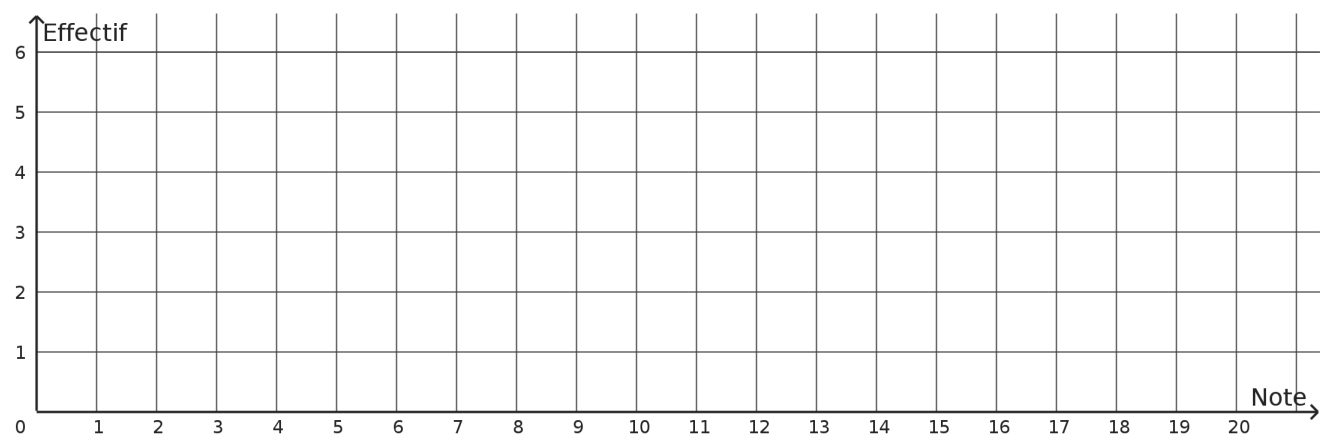
\includegraphics[width=\linewidth]{Images/DM1-graphique.png}
    \end{exercice}
    
    \begin{exercice}
    \brm{4}
        \begin{multicols}{2}
            \begin{center}
                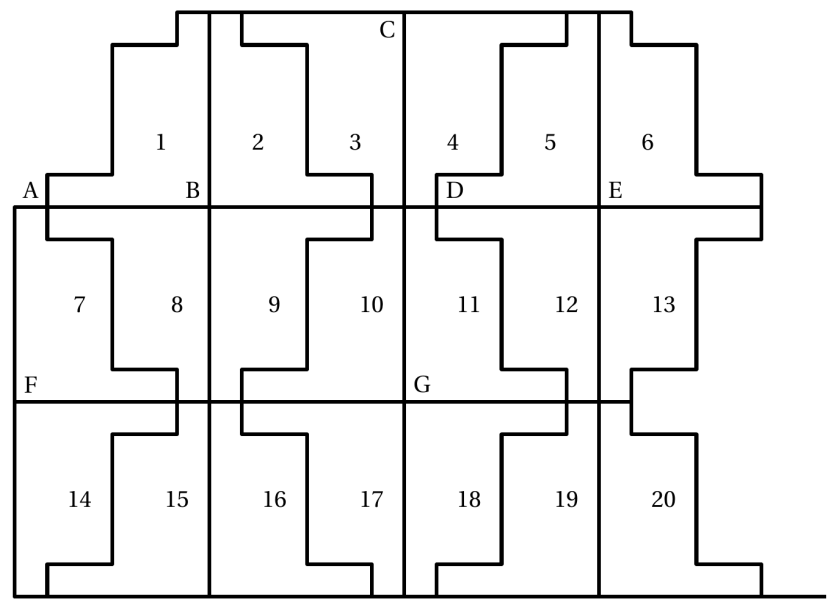
\includegraphics[width=\linewidth]{Images/DM1-exercice2.png}
            \end{center}
            
            \columnbreak
            Sans justifier, indiquer sur ta copie le numéro du motif qui convient :
            \begin{enumerate}
                \item Quelle est l’image du motif 1 par la translation qui transforme le point B en E ?
                \item Quelle est l’image du motif 1 par la symétrie de centre B ?
                \item Quelle est l’image du motif 16 par la symétrie de centre G ?
                \item Quelle est l’image du motif 2 par la symétrie d’axe (CG) ?
            \end{enumerate}
        \end{multicols}
    \end{exercice}

    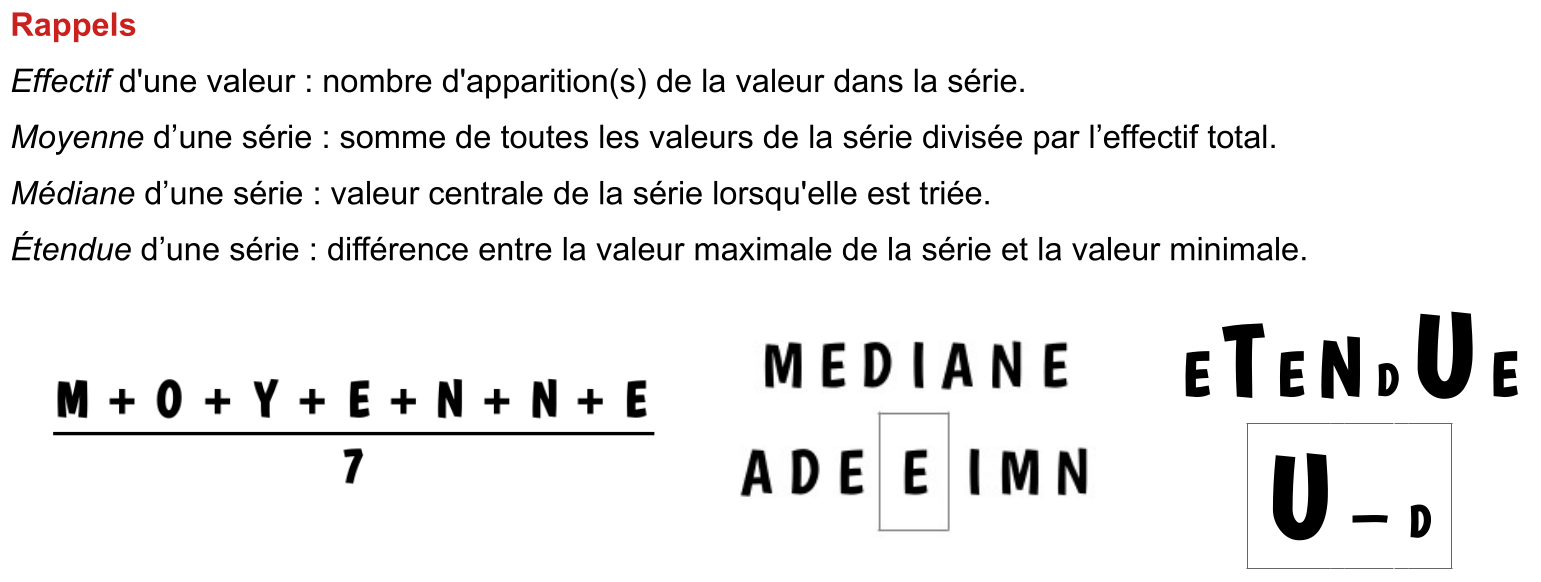
\includegraphics[width=.8\linewidth]{Images/RappelsStats.png}


\end{Maquette}


\end{document}